%%%%%%%%%%%%%%%%%%%%%%%%%%%%%%%%%%%%%%%%%%%%%%%%%%%%%%%%%%%%%%%%%%%%%%%%%%%%
% AGUJournalTemplate.tex: this template file is for articles formatted with LaTeX
%
% This file includes commands and instructions
% given in the order necessary to produce a final output that will
% satisfy AGU requirements, including customized APA reference formatting.
%
% You may copy this file and give it your
% article name, and enter your text.
%
% guidelines and troubleshooting are here:

%% To submit your paper:

\documentclass[draft]{agujournal2019}

\usepackage{url}
%this package should fix any errors with URLs in refs.
\usepackage{lineno}
\usepackage[inline]{trackchanges}
%for better track changes. finalnew option will compile document with changes incorporated.
\usepackage{soul}
\linenumbers % Adding packages
\usepackage{multirow}
\usepackage{colortbl}
\usepackage{amsmath}
\usepackage[separate-uncertainty = true,multi-part-units=single]{siunitx}
\usepackage[version=4]{mhchem}
\usepackage{booktabs}
% To thicken table lines
\usepackage{tikz}
\usetikzlibrary{arrows.meta}
%%%%%%%
% As of 2018 we recommend use of the TrackChanges package to mark revisions.
% The trackchanges package adds five new LaTeX commands:
%
%  \note[editor]{The note}
%  \annote[editor]{Text to annotate}{The note}
%  \add[editor]{Text to add}
%  \remove[editor]{Text to remove}
%  \change[editor]{Text to remove}{Text to add}
%
% complete documentation is here: http://trackchanges.sourceforge.net/
%%%%%%%

% \draftfalse

\journalname{JGR: Atmospheres}

\begin{document}
  \addeditor{eirik} \addeditor{reviewer1}

  %%%%%%%%%%%%%%%%%%%%%%%%%%%%%%%%%%%%%%%%%%%%%%%
  %  TITLE
  %
  % (A title should be specific, informative, and brief. Use
  % abbreviations only if they are defined in the abstract. Titles that
  % start with general keywords then specific terms are optimized in
  % searches)
  %
  %%%%%%%%%%%%%%%%%%%%%%%%%%%%%%%%%%%%%%%%%%%%%%%

  \title{Radiative forcing by supereruptions}

  %%%%%%%%%%%%%%%%%%%%%%%%%%%%%%%%%%%%%%%%%%%%%%%
  %
  %  AUTHORS AND AFFILIATIONS
  %
  %%%%%%%%%%%%%%%%%%%%%%%%%%%%%%%%%%%%%%%%%%%%%%%

  \authors{Eirik R. Enger\affil{1}, Rune Graversen\affil{1}, Audun Theodorsen\affil{1}}

  \affiliation{1}{UiT The Arctic University of Norway, Tromsø, Norway}

  \correspondingauthor{Eirik R. Enger}{eirik.r.enger@uit.no}

  \begin{keypoints}
    \item
    The ERF to AOD ratio has a time-after-eruption dependence on eruption latitude.
    \item
    No simulations across several climate models are found to produce ERF perturbations
    beyond \(\SI{-65}{\watt\meter^{-2}}\).
    \item
    Temperature and ERF peak values has a linear dependence with maximum temperature
    perturbations of \(\sim \SI{-10}{\kelvin}\).

    % \item
    % Model family is pivotal in determining estimated AOD and ERF from injected \ce{SO2},
    % while models generally demonstrate consistency in representing ERF from AOD.
  \end{keypoints}

  \begin{abstract}
    Volcanic activity causes cooling of the climate due to reflection of solar radiation
    by associated aerosols. The climate effect of an eruption may last for about a
    decade, but where the climate effect is only loosely tied to the magnitude of the
    eruption. We investigate the climatic effects of volcanic eruptions spanning from
    Mt.\ Pinatubo-sized events to supereruptions. The study is based on ensemble
    simulations in the Community Earth System Model Version 2 (CESM2) climate model
    applying the Whole Atmosphere Community Climate Model Version 6 (WACCM6) atmosphere
    model. Our analysis focuses on the impact of different \ce{SO2}-amount injections on
    stratospheric aerosol optical depth (AOD), effective radiative forcing (ERF), and
    global mean surface temperature (GMST) anomalies. We uncover a notable
    time-dependent decrease in aerosol forcing efficiency (ERF normalised by AOD) across
    all eruption magnitudes during the first post-eruption year. In addition, it is
    revealed that the largest eruptions investigated in this study, including several
    previous supereruption simulations, produces peak ERF anomalies bounded at
    \(\SI{-65}{\watt\meter^{-2}}\). Further, we find a close linear relationship between
    peek GMST and ERF, effectively bounding the GMST anomaly to at most
    \(\sim\SI{-10}{\kelvin}\). This is consistent across several previous studies using
    different climate models, while the largest uncertainty in model codes is found to
    relate to the chemistry and physics of aerosol evolution.
  \end{abstract}

  % Atmospheres now.
  % https://www.agu.org/Publish-with-AGU/Publish/Author-Resources/Text-requirements
  \section*{Plain Language Summary}

  % Here are instructions on writing a Plain Language Summary:
  % https://www.agu.org/Share-and-Advocate/Share/Community/Plain-language-summary

  Volcanic eruptions can have a significant impact on the Earth's climate. The gases
  from volcanic eruptions form aerosols. If the eruption is large enough, these aerosols
  may reach the stratosphere where they cause a cooling of the climate by reflecting
  sunlight. Typically, an eruption is distinguished by its impact on the opacity of the
  stratosphere and the change in the energy balance at the top of the atmosphere when
  the surface temperature is held fixed. The two measures are often assumed to be
  linearly related, but the linearity is useful only for eruptions of sizes seen in the
  last two millennia. We use a coupled climate model to simulate the impact of eruptions
  of sizes up to the largest known eruptions. The smallest eruptions we simulate are
  still large enough to cause global climate effects. In addition to the expected
  non-linear relationship between energy imbalance and stratospheric opacity for larger
  and larger eruptions, the ratio is found to also change over time. Additionally, we
  find evidence that the peak energy imbalance reaches a limit, and that the peak
  temperature response follows linearly with the peak energy imbalance, also reaching a
  limiting value.

  % NOTE: related to this, there is an index that can be added during publishing. Find
  % the list here:
  % https://www.agu.org/publish-with-agu/publish/author-resources/index-terms
  % 8409 - Atmospheric effects (0370)
  % 8408 - Volcano/climate interactions (1605, 3309, 4321)
  % 1627 - Coupled models of the climate system
  % 0305 - Aerosols and particles (0345, 4801, 4906)
  % 3363 - Stratospheric dynamics
  % 0370 - Volcanic effects

  \section{Introduction}

  % NOTE: Suggested layout for the introduction
  % - The objectives of the work.
  % - The justification for these objectives: Why is the work important?
  % - Background: Who else has done what? How? What have we done previously?
  % - Guidance to the reader: What should the reader watch for in the paper? What are the
  %   interesting high points? What strategy did we use?
  % - Summary/conclusion: What should the reader expect as conclusion? In advanced
  %   versions of the outline, you should also include all the sections that will go in
  %   the Experimental section (at the level of paragraph subheadings) and indicate what
  %   information will go.

  Stratospheric aerosol optical depth (AOD) and effective radiative forcing (ERF) are
  crucial metrics used to quantify the impact of major volcanic eruptions. The AOD
  represent the opacity of the stratosphere while ERF specifically is the energy
  imbalance at the top-of-atmosphere when ocean and sea-ice is held fixed. Radiative
  forcing can however be calculated differently, and an agreed-upon methodology has thus
  not always existed \cite{forster2016}. While ERF takes into account rapid adjustments,
  instantaneous radiative forcing (IRF) does not, with a third estimate of radiative
  forcing being a stratospherically adjusted radiative forcing where all surface and
  tropospheric conditions are kept fixed \cite{myhre2013,forster2016}. ERF, as used in
  this study, have been found to be the most precise indicator of the temperature
  response to a given forcing agent \cite{myhre2013,forster2016}, and a general
  assumption of a linear dependency of ERF on AOD is commonly adopted
  \cite{myhre2013,andersson2015}. Applying such a linear relationship has yielded
  reasonably accurate estimates in climate model simulations of volcanic eruptions
  \cite{mills2017,hansen2005,gregory2016,marshall2020,pitari2016b}. Yet, a wide spread
  in the estimated aerosol forcing efficiencies (ERF normalised by AOD) prevails among
  studies, spanning approximately from \(\sim \SI{-15}{\watt\metre^{-2}}\) per unit AOD
  (hereafter \(\si{\watt\metre^{-2}\mathrm{AOD}^{-1}}\)) \cite{pitari2016b} to
  \(\sim\SI{-25}{\watt\metre^{-2}\mathrm{AOD}^{-1}}\) \cite{hansen2005b}. Additionally,
  these estimates are predominantly based on small eruptions with AOD values up to at
  most \(\sim 0.7\).

  % the peak in AOD (at 500 nm) and thus the ERF depends also on the aerosol size
  % distribution, which evolves on a longer time scale than the conversion of SO2 to
  % aerosol.
  Although \ce{H2O}, \ce{N2}, and \ce{CO2} are the most abundant gases emitted by
  volcanoes \cite{robock2000}, sulphur species such as \ce{SO2} provide a comparatively
  greater influence due to the higher background concentrations of the former gases in
  the atmosphere. The transformation of \ce{SO2} molecules through reactions with
  \ce{OH} and \ce{H2O} leads to the formation of sulphuric acid (\ce{H2SO4})
  \cite{pinto1989,zhao1995}, which scatters sunlight thereby elevating planetary albedo
  and reducing the ERF. As the conversion from \ce{SO2} to \ce{H2SO4} occurs over weeks
  \cite{pinto1989,zhao1995}, the peak \ce{H2SO4} burden experiences a slight delay from
  the eruption's peak \ce{SO2} injection. The lifetime of the \ce{H2SO4} aerosols in the
  stratosphere depends on various factors, including aerosol size
  \cite{rampino1982,pinto1989,marshall2019}, latitude \cite{marshall2019, toohey2019},
  volcanic plume height \cite{marshall2019}, the quasi-biennial oscillation phase
  \cite{pitari2016b} and the season of the year (determining to which hemisphere
  aerosols are transported) \cite{toohey2011,toohey2019}. In the case of tropical
  eruptions, aerosols are typically transported poleward in the stratosphere and descend
  back to mid-latitude troposphere within one to two years \cite{robock2000}. Upon
  descending below the tropopause, these aerosols are readily removed by wet deposition
  \cite{liu2012}.

  Before the current era of significant anthropogenic climate forcing, volcanic
  eruptions were the primary forcing mechanism behind Earth's climate variability during
  the Holocene period \cite{schurer2013}. Despite this substantial impact, few
  climate-model experiments have included volcanic forcing when simulating climate
  evolution during the Holocene \cite{sigl2022}, likely implying an exaggerated positive
  forcing \cite{gregory2016,solomon2011}. This absence of persistent cooling is one of
  several factors that have been suggested to contribute to the common disparity between
  simulated and observed global warming \cite{andersson2015}. Despite extensive
  attention on understanding the way volcanic eruptions influence climate, questions
  regarding aerosol particle processes---such as growth and creation rates when \ce{OH}
  is scarce---remain unanswered
  \cite<e.g.~>[]{zanchettin2019,marshall2020,marshall2022,mcgraw2024}. These processes
  impact aerosol scattering efficiency and potentially the ERF to AOD relationship.
  \citeA{marshall2020} observe higher aerosol forcing efficiency in post-eruption years
  \(2\) and \(3\) compared to year 1, and attribute this post-eruption increase in
  aerosol forcing efficiency to strong spatial concentration in the initial year and
  subsequent distribution of aerosols over a larger area. This spatial redistribution
  increases the albedo per global mean AOD thereby causing a stronger ERF to AOD ratio
  \cite{marshall2020}.

  Previous studies of both Mt.\ Pinatubo \cite{mills2017,hansen2005} and volcanoes
  within the instrumental era \cite{gregory2016} have been used to estimate the
  relationship between the ERF energy imbalance and change in AOD. While
  \citeA{myhre2013} employ a formula scaling ERF by AOD to obtain
  \(\SI{-25}{\watt\metre^{-2}\mathrm{AOD}^{-1}}\), recent literature reports estimates
  as small as {\(\SI{-19.0(5)}{\watt\metre^{-2}\mathrm{AOD}^{-1}}\)} \cite{gregory2016}
  and \(\SI{-18.3(10)}{\watt\metre^{-2}\mathrm{AOD}^{-1}}\) \cite{mills2017}. Synthetic
  volcano simulations in \citeA{marshall2020} yield a scaling factor of
  \(\SI{-20.5(2)}{\watt\metre^{-2}\mathrm{AOD}^{-1}}\) across an ensemble of \(82\)
  simulations featuring varying injection heights and latitudes of volcanic emissions,
  with injected \ce{SO2} ranging from \(10\) to \(\SI{100}{\tera\gram(\ce{SO2})}\).

  A similar simulation setup, albeit with notable differences, was conducted by
  \citeA{niemeier2015}, involving an ensemble of \(14\) levels of injected sulphur
  spanning between \(\SI{1}{\tera\gram(\ce{S})\mathrm{yr}^{-1}}\)
  (\(\SI{2}{\tera\gram(\ce{SO2})\mathrm{yr}^{-1}}\)) and
  \(\SI{100}{\tera\gram(\ce{S})\mathrm{yr}^{-1}}\)
  (\(\SI{200}{\tera\gram(\ce{SO2})\mathrm{yr}^{-1}}\)). These geoengineering simulations
  maintained continuous sulphur injections, running until a steady sulphur level was
  achieved. Results indicated an inverse exponential relationship between maximum
  forcing and annually injected \ce{SO2}, converging to \(\SI{-65}{\watt\metre^{-2}}\)
  (Eq.~\ref{eq:niemeier_exponential}). Even the \(100\times\) Mt.\ Pinatubo
  supereruption simulation by \citeA{jones2005}, which obtained a peak ERF of
  \(\SI{-60}{\watt\metre^{-2}}\), is below the suggested limit of
  \(\SI{-65}{\watt\metre^{-2}}\). Moreover, \citeA{timmreck2010} find a peak ERF anomaly
  of \(\SI{-18}{\watt\metre^{-2}}\) from a \(\SI{1700}{\tera\gram(\ce{SO2})}\) eruption
  simulation, which corresponds well with the function estimated by \citeA{niemeier2015}
  at an annual injecting rate of
  \(\SI{1700}{\tera\gram(\mathrm{SO_2})\mathrm{yr}^{-1}}\). Several studies have
  demonstrated a linear relationship of approximately
  \(-\SI{20}{\watt\metre^{-2}\mathrm{AOD}^{-1}}\) between ERF and AOD, although
  substantial variability exists in the slope among studies
  \cite{mills2017,hansen2005,gregory2016,marshall2020,pitari2016b}. Moreover, a
  time-after-eruption dependence on the ERF to AOD ratio is found in
  \citeA{marshall2020}, whereas \citeA{niemeier2015} revealed a non-linear relationship
  between ERF and injected \ce{SO2} rate. Thus, a consensus on the relationship between
  injected \ce{SO2}, AOD, and ERF has yet to be established.

  One avenue that has garnered considerable attention is comparing the magnitude of
  volcanic or volcano-like forcings to increased \ce{CO2} levels. Several studies
  explore the connection between volcanic forcing and the climate sensitivity to a
  doubling of \ce{CO2}
  \cite{boer2007,marvel2016,merlis2014,ollila2016,richardson2019,salvi2022,wigley2005}.
  The comparison of forcing from volcanoes and \ce{CO2} aims to mitigate the large
  uncertainty in estimates of the sensitivity of the real climate system. Inferring
  climate sensitivity from volcanic eruption events has been attempted as a way to
  constrain the sensitivity \cite{boer2007} by assuming that volcanic and \ce{CO2}
  forcings produce similar feedbacks \cite{pauling2023}. Earlier studies suggest the
  potential for constraining equilibrium cilmate sensitivity (ECS) using volcanoes
  \cite{bender2010}, provided that ECS is constrained by ERF rather than IRF, as ERF
  accounts for rapid atmospheric adjustments in contrast to IRF
  \cite{smith2018,richardson2019,marshall2020}. However, other studies refute this
  approach, pointing out that different sensitivities of volcanic forcing and \ce{CO2}
  doubling seem to exist \cite{douglass2006}, or that constraining the ECS by ERF lacks
  accuracy due to the precision of climate simulations \cite{boer2007,salvi2022}.
  Although ERF offers a more suitable indicator of forcing than IRF
  \cite{marvel2016,richardson2019}, more recent studies conclude that ECS cannot be
  constrained from volcanic eruption events \cite{pauling2023}.

  Employing eruptions about an order of magnitude or more greater than the Mt.\ Pinatubo
  eruption (Volcano-Climate Index value greater than \(3\) \cite{schmidt2022}) enhances
  the signal-to-noise ratio without necessitating an extensive and computationally
  expensive ensemble, and as such, is a tempting shortcut to try and mimic a large
  ensemble of smaller volcanic eruptions. However, the AOD, ERF, and GMST signatures are
  not necessarily a simple scaling of that of smaller volcanic eruptions. Previous
  studies have simulated supereruptions using AOD as the input forcing, where the AOD
  was that of Mt.\ Pinatubo scaled by a factor of one hundred \cite{jones2005}. More
  recent studies find this approach will yield incorrect results, because the peak of
  the AOD is likely to be too large, and the evolution of the AOD could be inappropriate
  due to \ce{OH} scarcity and aerosol size \cite{timmreck2009,timmreck2010}. Likewise, a
  different AOD evolution may be found from similar size eruptions, but at different
  latitudes \cite{schneider2009,marshall2020,zhuo2024}. To investigate the climate
  effects of large, Mt.\ Pinatubo-like, eruptions compared to supereruptions, as well as
  latitudinal effects, our simulations are based on four levels of injected \ce{SO2}
  covering three orders of magnitude and the inclusion of one high latitude eruption of
  the second largest injected \ce{SO2} case.

  We conducted ensemble simulations of volcanic eruptions in the Community Earth System
  Model Version 2 (CESM2) coupled with the Whole Atmosphere Community Climate Model
  Version 6 (WACCM6). The ensembles span four different levels of injected \ce{SO2}:
  \(\SI{26}{\tera\gram(\ce{SO2})}\), \(\SI{400}{\tera\gram(\ce{SO2})}\),
  \(\SI{1629}{\tera\gram(\ce{SO2})}\) and \(\SI{3000}{\tera\gram(\ce{SO2})}\). Details
  regarding the experimental setup are provided in section~\ref{sec:method}. Our
  findings reveal non-linear ERF to AOD dependencies for large to super-volcano size
  eruptions. Additionally, we observe a time-dependent variation in the ERF to AOD
  ratio, detailed in section~\ref{sec:results} and discussed in
  section~\ref{sec:discussion}. Furthermore, our data, along with insights from previous
  studies, suggest that the ERF dependency on injected \ce{SO2} identified by
  \citeA{niemeier2015} acts as a lower boundary. Our conclusions are presented in
  section~\ref{sec:conclusions}.

  \section{Method}

  \label{sec:method}

  \subsection{Model}

  We use the CESM2 \cite{danabasoglu2020} in conjunction with the WACCM6
  \cite{gettleman2019} and the fully dynamical ocean component Parallel Ocean Program
  version 2 (POP2) \cite{smith2010, danabasoglu2020}. The atmosphere model was run at a
  nominal \(\SI{2}{\degree}\) resolution with \(70\) vertical levels in the middle
  atmosphere (MA) configuration.

  The WACCM6 version employed in the MA configuration uses the three mode version of the
  Modal Aerosol Module (MAM3) \cite{gettleman2019}, a simplified and computationally
  efficient default setting within the Community Atmosphere Model version 5 (CAM5)
  \cite{liu2016}, as described in \citeA{liu2012}. The MAM3 was developed from MAM7 and
  features the modes Aitken, accumulation, and coarse \cite{liu2016}, and further
  updated to simulate stratospheric sulfate aerosol from volcanic and non-volcanic
  emissions in WACCM \cite{mills2016}.

  \subsection{Simulations}

  We are using the coupled model version BWma1850 component setup to run the CESM2 with
  a fully dynamic ocean component to get estimates of the GMST, and an accompanying
  fixed sea-surface temperature version, fSST1850, providing estimates of the ERF and
  AOD. The applied fSST1850 is not from a standardised component setup of CESM2 but is
  instead explicitly specified as \url{1850_CAM60
    %WCCM_CLM50%BGC-CROP_CICE%PRES_DOCN%DOM_MOSART_CISM2%NOEVOLVE_SWAV_TEST
    %
  }. % Necessary to make the formatter not break the URL / literal text
  The component setup BWma1850 and fSST1850 differ in that the latter uses a prescribed
  sea-ice (\texttt{CICE -> CICE\%PRES}), a prescribed data ocean (\texttt{POP2\%ECO\%DEP
    -> DOCN\%DOM}) and a stub wave component instead of the full Wave Watch version 3
  (\texttt{WW3 -> SWAV}).

  The important input data used in the model simulations are injected \ce{SO2} in units
  of teragrams (\(\si{\tera\gram(\ce{SO2})}\)), used to simulate volcanic eruptions. ERF
  is calculated as the combined (short wave and long wave) all-sky TOA energy imbalance,
  where the CESM2 provide the output variables ``net solar flux at the top of the
  model'' (FSNT) and ``net longwave flux at the top of the model'' (FLNT). Thus,
  \(\mathrm{ERF_*}= \mathrm{FSNT} - \mathrm{FLNT}\), and taking the difference between
  volcanic forcing simulations and a control simulation gives the final estimate of ERF
  (\(\mathrm{ERF}=\mathrm{ERF_{VOLC}}-\mathrm{ERF_{CONTROL}}\)) \cite{marshall2020}. The
  ERF calculation uses the fSST1850 component setup, which is also used to obtain all
  other simulation output fields except from GMST which uses BWma1850. The AOD is
  obtained from the output variable ``stratospheric aerosol optical depth 550 nm day
  night'' (AODVISstdn), while GMST is saved by CESM2 to the variable ``reference height
  temperature'' (TREFHT). The analysis of this work is performed using these four
  variables.

  Appendix A provides a description of the simulation setup.
  Table~\ref{tab:simulation-overview} summarises the simulations, encompassing four
  \ce{SO2} injection magnitudes and up to four seasons: 15 February, 15 May, 15 August,
  and 15 November. The magnitudes vary over three orders of magnitude, or as introduced
  in \citeA{schmidt2022} across Volcano-Climate Index values \(3\) to \(6\):
  \(\SI{26}{\tera\gram(\ce{SO2})}\), \(\SI{400}{\tera\gram(\ce{SO2})}\),
  \(\SI{1629}{\tera\gram(\ce{SO2})}\), and \(\SI{3000}{\tera\gram(\ce{SO2})}\).

  The smallest eruption case, S26, is similar in magnitude as compared to events like
  Mt.\ Pinatubo \cite<\(\sim10\)--\(\SI{20}{\tera\gram(\ce{SO2})}\);>[]{timmreck2018}
  and Mt.\ Tambora \cite<\(\sim\SI{56.2}{\tera\gram(\ce{SO2})}\);>[]{zanchettin2016}.
  The intermediate case, S400, resembles the magnitude of the Samalas eruption in 1257
  \cite<\(\sim{144}\)--\(\SI{170}{\tera\gram(\ce{SO2})}\);>[]{vidal2016} however
  injecting about twice of the estimated \ce{SO2}, while the second largest and largest
  eruption cases, S1629 and S3000, is in the likely range of the Young Toba Tuff (YTT)
  supereruption occurring about \(\SI{72000}{\mathrm{yr}}\) ago
  \cite<\(100\)--\(\SI{10000}{\tera\gram(\ce{SO2})}\);>[]{jones2005}. All eruptions were
  situated at the equator (\(\SI{0}{\degree N}\), \(\SI{1}{\degree E}\)) with \ce{SO2}
  injected from \(\SI{18}{\kilo\meter}\) to \(\SI{20}{\kilo\meter}\) altitude with a
  linear ramp; 25\% between \(\SI{17.5}{\kilo\meter}\) and \(\SI{18.5}{\kilo\meter}\),
  50\% between \(\SI{18.5}{\kilo\meter}\) and \(\SI{19.5}{\kilo\meter}\), and the last
  25\% between \(\SI{19.5}{\kilo\meter}\) and \(\SI{20.5}{\kilo\meter}\). Collectively,
  the four tropical eruption cases S26, S400, S1629, and S3000 are referred to as STrop.
  An additional high-latitude eruption ensemble, labelled S1629N, of the same injected
  \ce{SO2} magnitude as S1629 was simulated at \(\SI{56}{\degree N}\),
  \(\SI{287.7}{\degree E}\) with a six-month separation (15 February and 15 August)
  between the two simulations.

  \begin{table*}
    \centering

    \caption{Simulations done with the CESM2\(^{a}\)}\label{tab:simulation-overview}%
    \begin{center}
      \begin{tabular}[c]{cccccc}
        \toprule
        Ensemble name & \(\si{\tera\gram(\ce{SO2})}\) &
        Lat [\si{\degree\mathrm{N}}] & Lon [\si{\degree\mathrm{E}}] & Alt [\si{\kilo\metre}] & Eruption months \\
        \midrule
        S3000 & \(3000\) &
        \(\hphantom{1}0\) & \(\hphantom{28}1\hphantom{.7}\) &
        \(18\)--\(20\) & \hphantom{Feb,}May,\hphantom{Aug,}Nov \\
        S1629N & \(1629\) &
        \(56\) & \(287.7\) &
        \(18\)--\(20\) & Feb,\hphantom{May,}Aug\hphantom{,Nov} \\
        S1629 & \(1629\) &
        \(\hphantom{1}0\) & \(\hphantom{28}1\hphantom{.7}\) & \(18\)--\(20\)
        & Feb,May,Aug,Nov \\
        S400 & \(\hphantom{1}400\) &
        \(\hphantom{1}0\) &
        \(\hphantom{28}1\hphantom{.7}\) &
        \(18\)--\(20\) & Feb,May,Aug,Nov \\
        S26 & \(\hphantom{14}26\) &
        \(\hphantom{1}0\) &
        \(\hphantom{28}1\hphantom{.7}\) & \(18\)--\(20\)
        &
        Feb,May,Aug,Nov \\
        \toprule
        \multicolumn{6}{l}{\parbox{\linewidth}{\(^{a}\)The ensembles S1629N and S1629
            have the same eruption magnitude, but while S1629 is located at the equator,
            S1629N is located at a high northern latitude. S3000, S400 and S26 are
            located at the equator, but with different magnitudes compared to S1629. The
            three smallest in eruption magnitude tropical ensembles have four members,
            indicated by the number of eruption months, while ensembles S1629N and S3000
            consist of two members.}}
      \end{tabular}
    \end{center}
  \end{table*}

  \section{Results}

  \label{sec:results}

  % NOTE: the results should be laid out in a logical way, with the most
  % interesting/important stuff first, then tangents that dig deeper at specific things
  % later.
  % 1. ERF to AOD time-after-eruption dependence should be top priority (8 figs atm.)
  % 2. Then probably temperature scaling since we discuss the shape of both AOD and ERF
  %    time series before that (MOTIVATION: can we expect a specific temperature time
  %    series shape based on the shape of either of or both of the ERF and AOD time
  %    series?)
  % 3. If there is something interesting to say about the rest of the figures (all the
  %    comparing of parameters), then this should come here.

  \subsection{Analysis of the time series}

  Figure~\ref{fig:1_compare_waveform} presents time series of global mean AOD, ERF, and
  GMST. The black lines represent the medians across the ensembles, while shading
  indicates the 5th to 95th percentiles. The four distinct forcing magnitudes (S26,
  S400, S1629, and S3000) outlined in table~\ref{tab:simulation-overview} have been
  used. The time series in Fig.~\ref{fig:1_compare_waveform} are normalised by setting
  the peak value to unity, defined based on the peak of a fit from a Savitzky-Golay
  filter of 3rd order and a one-year window length \cite{savitzky1964}.

  A notable feature across the subfigures of Fig.~\ref{fig:1_compare_waveform} is the
  peak occurrence of the S26 case compared to the larger eruption cases. The peak of S26
  arrives earlier for both normalised AOD (Fig.~\ref{fig:1_compare_waveform}a) and
  normalised GMST (Fig.~\ref{fig:1_compare_waveform}c), while the normalised ERF time
  series in Fig.~\ref{fig:1_compare_waveform}b are all indistinguishable. Cases S400,
  S1629, and S3000 are indistinguishable in their normalised GMST development, and while
  S26 peaks at an earlier time, it decays similarly to the other cases. Interestingly,
  the same development between S400 and S1629 is not found in the normalised AOD time
  series. S26 peaks at an earlier time, but also spends more time around the peak and as
  such decays at a later time post-eruption. Likewise, S400 has a faster rise and slower
  decay compared to S1629, but where both peak at a similar time. S1629 and S3000 have
  similar normalised AOD developments, but where S3000 show a slightly faster decay from
  the peak.

  The timescale of the perturbation of AOD and ERF is shorter than that of the GMST.
  While the AOD and ERF time series return to their equilibrium state within roughly
  three years, the GMST time series remain heavily perturbed three years post-eruption.
  Even when running the simulations for 20 years post-eruption, the GMST time series are
  still decaying.

  \begin{figure}
    \centering 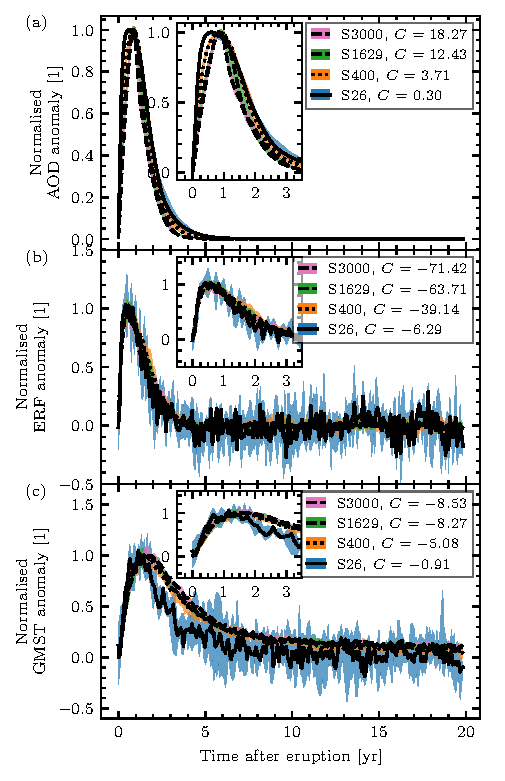
\includegraphics{figure1}

    \caption{AOD (a), ERF (b) and GMST response (c) time series to the four tropical
      volcanic eruption cases, S26, S400, S1629, and S3000. The time series have been
      normalised to have peak values at unity, where \(C\) is the normalisation
      constant. Black lines indicate the median across the ensembles, while shading
      marks the 5th and 95th percentiles.}\label{fig:1_compare_waveform}%
  \end{figure}

  \subsection{ERF dependency on AOD}

  We next focus on the development of the AOD and ERF time series relative to each
  other. Similar comparisons were conducted in \citeA<>[their Fig.\ 4]{gregory2016} and
  \citeA<>[their Fig.\ 1]{marshall2020}, with ERF plotted against AOD.
  Figure~\ref{fig:2_rf_vs_aod_slopes} displays annual mean values from the five
  simulation cases in table~\ref{tab:simulation-overview}; S26 as blue downward-pointing
  triangles, S400 as orange thick diamonds, S1629 as green upward-pointing triangles,
  S3000 as small pink upward-pointing carets, and S1629N as brown upward-pointing
  three-branched twigs. Also shown are the data from \citeA<>[Fig.\ 4, black
    crosses]{gregory2016} as grey crosses labelled G16 (described in Appendix B,
  section~\ref{ap:g16}). Additionally, the estimated peak values from the Mt.\ Pinatubo
  and Mt.\ Tambora eruptions are plotted as a black star and plus, while the peak from
  the \citeA{jones2005} simulation is shown as a pink square labelled J05. Finally, red
  circles represent the peak values obtained from the STrop eruption cases. The straight
  lines are the same as shown by \citeA{gregory2016}. The full data range is shown in
  Fig.~\ref{fig:2_rf_vs_aod_slopes}a while Fig.~\ref{fig:2_rf_vs_aod_slopes}b highlights
  a narrow range, focusing on S26.

  The annual mean data from the Mt.\ Pinatubo-like S26 case in
  Fig.~\ref{fig:2_rf_vs_aod_slopes}b have ERF values as a function of AOD that follow
  almost the same constant slope as the G16 data. However, in
  Fig.~\ref{fig:2_rf_vs_aod_slopes}a we observe that the stronger eruptions lead to
  dissimilar responses in AOD and ERF, where S400 seems to follow close to a \(-10\)
  slope and S1629 is closer to a \(-5\) slope. The peak values (red circles) suggest a
  non-linear dependence, while within each eruption strength (same colour) the annual
  mean values fall relatively close to a straight line.

  \begin{figure}
    \centering 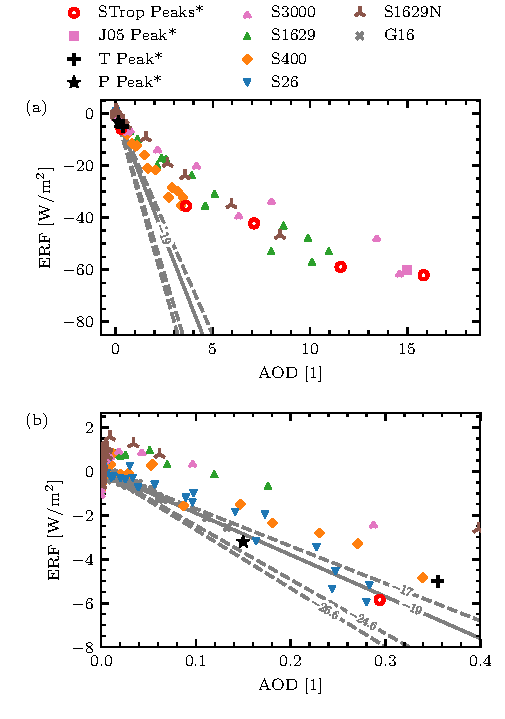
\includegraphics{figure2}

    \caption{ERF as a function of AOD, yearly means. Data from the five simulations
      listed in table~\ref{tab:simulation-overview} (S26, S400, S1629, S1629N, and
      S3000) are shown along with the data from the HadCM3 simulation by
      \citeA{gregory2016} (grey crosses, G16). Also shown are the estimated peak values
      of the Mt.\ Pinatubo (black star) and Mt.\ Tambora (black plus) eruptions. The
      peak values from the STrop simulations are shown as red circles. Additionally in
      (a) the simulated super-volcano of \citeA{jones2005} (pink square) is shown. All
      peak values (as opposed to annual means) have an asterisk (\(\ast{}\)) in their
      label. The grey lines are the same regression fits as in \citeA<>[Fig.\
        4]{gregory2016}, where the solid line is the fit to G16. (b): Zooming in on the
      smallest AOD values.}\label{fig:2_rf_vs_aod_slopes}%
  \end{figure}

  To investigate the time dependence of the ratio between ERF and AOD, we present
  seasonal means of this ratio in Fig.~\ref{fig:3_rf_to_aod_ratios}. The plot shows the
  eruption cases given in table~\ref{tab:simulation-overview}, as well as the tropical
  eruptions from \citeA{marshall2020dataset} (\(6\) of \(82\) eruptions), labelled M20
  and described in Appendix B, section~\ref{ap:m20}. The S1629 case is similar to S3000
  as indicated in table~\ref{tab:slope-gradients}, but is not shown in the plot to
  better highlight S1629N. In Fig.~\ref{fig:3_rf_to_aod_ratios}a, lines are linear
  regression fits to the seasonal means across all ensemble members, summarised in
  table~\ref{tab:slope-gradients}. Shaded regions are the standard deviation around the
  seasonal means. A similar plot is presented in Fig.~\ref{fig:3_rf_to_aod_ratios}b, but
  where the AOD and ERF time series were scaled to have peak values at unity before
  computing the ratio. As the AOD and ERF time series start from zero, the ratio from
  the first season is not included. Likewise, after three years both time series are
  almost fully equilibrated (Fig.~\ref{fig:1_compare_waveform}a,b). The data is further
  divided into two periods; a pre-peak period where the peak of both the AOD and the ERF
  is included (consisting of the first post-eruption year), and a post-peak period for
  the decaying part (consisting of the second and third post-eruption years).

  Although the ratio changes across the eruption magnitudes, we find that all the
  tropical cases follow a positive slope during the pre-peak period, as seen in
  Fig.~\ref{fig:3_rf_to_aod_ratios}a and described in table~\ref{tab:slope-gradients}.
  The northern latitude case in S1629N shows a much flatter slope compared to STrop and
  M20. The distinction between the slopes from the tropical and non-tropical cases is
  perhaps more clear in Fig.~\ref{fig:3_rf_to_aod_ratios}b and corresponding rows in
  table~\ref{tab:slope-gradients}. Again, S1629N shows an almost flat slope compared to
  the tropical cases. During the post-peak period, more noise is introduced, but a weak
  tendency of negative slopes is found among the tropical cases, as well as in the
  S1629N case up to the last season where the noise is also the largest.

  \begin{table}
    \centering

    \caption{Slope and standard deviation for the data in
      Fig.~\ref{fig:3_rf_to_aod_ratios}\(^{a}\)}\label{tab:slope-gradients}%
    \begin{tabular}{cccc}
      \toprule
      Figure & Ensemble name & Pre-peak & Post-peak \\
      \midrule
      & S1629N & \(0.45\pm1.15\) & \(1.51\pm1.45\) \\
      & S3000 & \(3.38\pm0.97\) & \(-2.74\pm0.77\) \\
      \multirow{2}{*}{\ref{fig:3_rf_to_aod_ratios}a} & S1629 & \(3.85\pm0.52\) & \(-3.29\pm0.60\) \\
      & S400 & \(4.36\pm0.82\) & \(-3.37\pm0.59\) \\
      & S26 & \(3.64\pm2.41\) & \(-1.41\pm3.25\) \\
      & M20 & \(6.34\pm1.77\) & \(-0.36\pm1.33\) \\
      \midrule
      & S1629N & \(0.08\pm0.20\) & \(0.27\pm0.26\) \\
      & S3000 & \(0.86\pm0.25\) & \(-0.70\pm0.19\) \\
      \multirow{2}{*}{\ref{fig:3_rf_to_aod_ratios}b} & S1629 & \(0.75\pm0.10\) & \(-0.64\pm0.12\) \\
      & S400 & \(0.43\pm0.08\) & \(-0.34\pm0.06\) \\
      & S26 & \(0.18\pm0.12\) & \(-0.07\pm0.16\) \\
      & M20 & \(0.33\pm0.07\) & \(-0.02\pm0.08\) \\
      \toprule
      \multicolumn{4}{l}{\parbox{0.6\linewidth}{\(^{a}\)The regression fits in the top half of the table are for
          Fig.~\ref{fig:3_rf_to_aod_ratios}a, while the bottom half is for
          Fig.~\ref{fig:3_rf_to_aod_ratios}b. The columns ``pre-peak'' and ``post-peak'' refer to
          the two periods as shown in Fig.~\ref{fig:3_rf_to_aod_ratios}. The ensembles are the
          same as those given in table~\ref{tab:simulation-overview}, in addition to the \(6\)
          tropical eruptions from the \(82\) member ensemble in
          \citeA{marshall2020}.}} \\
    \end{tabular}
  \end{table}

  \citeA<>[their Fig.\ 1c,d]{marshall2020} present results that demonstrate a
  time-dependent relationship in the conversion between AOD and ERF. They obtain an ERF
  to AOD ratio with a negative slope when comparing the first post-eruption year to the
  second and third. As such, \citeA{marshall2020} find that, on average, the aerosol
  forcing efficiency increases during the first two to three post-eruption years. This
  phenomenon is explained by \citeA{marshall2020} as the aerosols initially being
  spatially confined to the hemisphere where the eruption occurred. Subsequently, during
  the second and third years, they spread globally, resulting in a higher global-mean
  albedo per AOD and consequently a stronger ERF per AOD ratio with time. However, as
  noted above, a decrease in aerosol forcing efficiency is found when analysing the M20
  data with seasonal resolution during the pre-peak period (first year post-eruption)
  while constraining the ensemble to only include eruptions within \(-10\) to
  \(\SI{10}{\degree\mathrm{N}}\). The post-peak period shows an increasing aerosol
  forcing efficiency, and during the full first three post-eruption years (pre-peak and
  post-peak), both the tropical subset and the full M20 data yield an increasing
  efficiency, as expected. Likewise, the first three post-eruption years of the S400,
  S3000, and S1629N cases show a weak negative slope and thus an increasing efficiency,
  while S26 shows an elevated post-peak ratio as seen in
  Fig.~\ref{fig:3_rf_to_aod_ratios}b.

  We also note that while the aerosol forcing efficiency is decreasing for tropical M20
  data in the pre-peak period, the full dataset shows increasing efficiency. This is in
  line with what we find from S1629N, which is the only eruption case that does not show
  a clear aerosol forcing efficiency decrease during the pre-peak period.

  \begin{figure}
    \centering 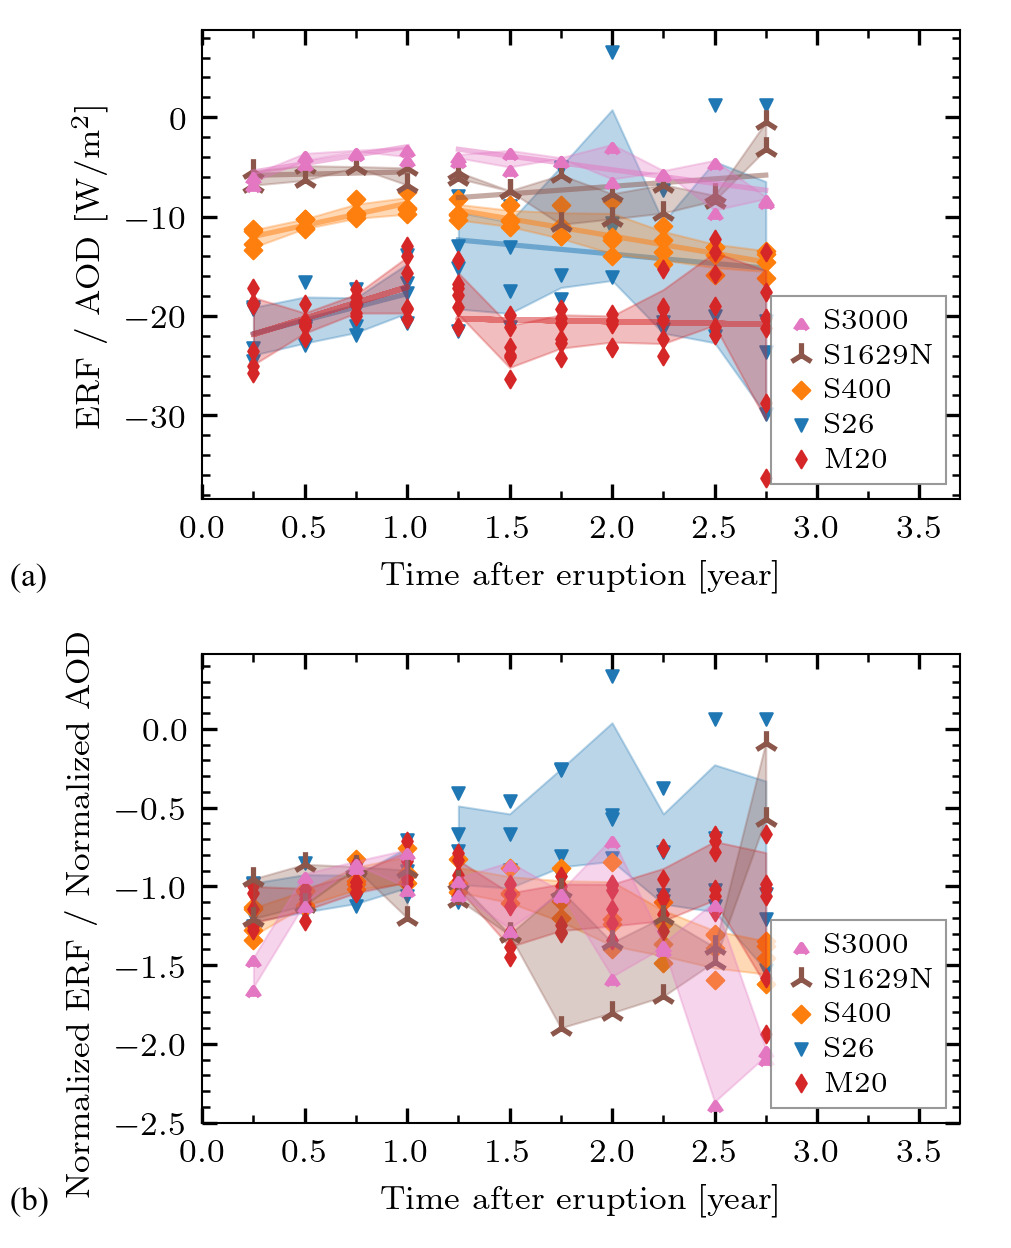
\includegraphics{figure3}

    \caption{(a): The ratio of ERF to AOD, with time-after-eruption on the horizontal
      axis. Straight lines indicate linear regression fits and are described in
      table~\ref{tab:slope-gradients}, while shaded regions are the standard deviation
      across the ensembles for each season. Regression fits and shadings are made for
      the pre-peak and post-peak periods. (b): Same as in (a), but where the underlying
      AOD and ERF time series have been scaled to have peak values at unity. Shown are
      data from table~\ref{tab:simulation-overview} along with tropical eruptions from
      M20. Values from each ensemble member is omitted for clarity, but we note that S26
      include some outliers at positive ratio after the start of the second
      post-eruption year.}\label{fig:3_rf_to_aod_ratios}%
  \end{figure}

  \subsection{Parameter scan}

  In Fig.~\ref{fig:4_parameter_scan}, we compare the peak values of all investigated
  CESM2 output parameters against each other as well as to injected \ce{SO2}, grouped
  into tropical cases (STrop) and the high-latitude case (S1629N). We also include data
  from \citeA{marshall2020} (M20); \citeA{jones2005} (J05); \citeA{timmreck2010} (T10);
  \citeA{english2013} (E13); \citeA{niemeier2015} (N15); \citeA{ottobliesner2016}
  (OB16); \citeA{brenna2020} (B20); \citeA{osipov2020} (Os20); and \citeA{mcgraw2024}
  (McG24). A description of the climate models used is presented in
  table~\ref{tab:model-family}. Additionally, peak values from Mt.\ Pinatubo (P) and
  Mt.\ Tambora (T) are shown for reference.

  For STrop, we observe in Fig.~\ref{fig:4_parameter_scan}a an almost linear yet notably
  weakening relationship between AOD peak values and injected \ce{SO2}. The latitude
  also plays a role in the magnitude of the AOD perturbation, evident from S1629N. This
  weak yet notable latitude dependence aligns with findings by \citeA{marshall2019},
  indicating that \(\SI{72}{\percent}\) of the AOD variance can be attributed to
  injected \ce{SO2}, while latitude accounts for only \(\SI{16}{\percent}\) of the
  variance. Peak values from their data (82 simulations) plotted as red thin diamonds
  display a similar pattern, with AOD exhibiting close to linear dependence on injected
  \ce{SO2}, but with latitude introducing a spread in AOD. Peak values from
  Mt.\ Pinatubo (P) and Mt.\ Tambora (T) align well with simulation data, while peak
  values from other simulations of large \ce{SO2} magnitudes (J05, E13, T10, Os20) show
  a larger spread, specifically to weaker AOD response. B20 align well with STrop, which
  also used the CESM2(WACCM6) climate model. Even though E13 used a similar yet simpler
  and older model in WACCM3 as compared to the CESM2(WACCM6) used by B20 and here, their
  AOD peak values are significantly smaller. However, E13 obtained significantly larger
  aerosols than B20; from an eruption injecting
  \(\SI{2000}{\tera\gram(\mathrm{SO_{2}})}\) E13 find a peak aerosol effective radius of
  \(R_{\mathrm{EFF}}=\SI{1.9}{\micro\meter}\), while B20 obtained
  \(R_{\mathrm{EFF}}=\SI{0.7}{\micro\meter}\) from an eruption injecting half as much
  \ce{SO2}. Also shown is the two-thirds power-law relationship between AOD and injected
  \ce{SO2} suggested by \citeA{crowley2013}, scaled to yield the same value in AOD for
  an injection of \(\SI{3000}{\tera\gram(\mathrm{SO_{2}})}\) as obtained by S3000.

  In Fig.~\ref{fig:4_parameter_scan}b, ERF plotted against injected \ce{SO2} (with the
  absolute value of ERF on the \(y\)-axis) show a sublinear ERF increase with increasing
  injected \ce{SO2}, in part due to the increase in aerosol effective radius with
  increasing eruption magnitudes \cite{timmreck2009}. This damping effect is seen in the
  STrop data to be in agreement with results from J05, B20, and McG24. While B20 uses
  the same climate model as STrop, McG24 uses the GISS ModelE2.1 but where a fixed
  aerosol effective radius of \(R_{\text{EFF}}=\SI{0.6}{\micro\meter}\) was used. This
  \(R_{\text{EFF}}\) is at the lower end of their simulations, which is shown by
  \citeA{mcgraw2024} to produce the most extreme ERF and GMST perturbations. J05 used a
  third climate model in HadCM3, but simulates from the AOD estimate of Mt.\ Pinatubo
  multiplied by \(100\), and thus also assume small aerosol effective radius. The OB16
  data come from a \(2500\) year long simulation using historic volcanoes as the only
  external forcing. The analysis details of OB16 can be found in Appendix B,
  section~\ref{ap:ob16}. Despite the model complexity difference as compared to STrop,
  \citeA{ottobliesner2016}'s simulations using Community Earth System Model version 1
  (CESM1) with a low-top atmosphere (CAM5) produce ERFs comparable to our findings, also
  aligning well with the synthetic simulations of M20.

  \begin{figure*}
    \centering 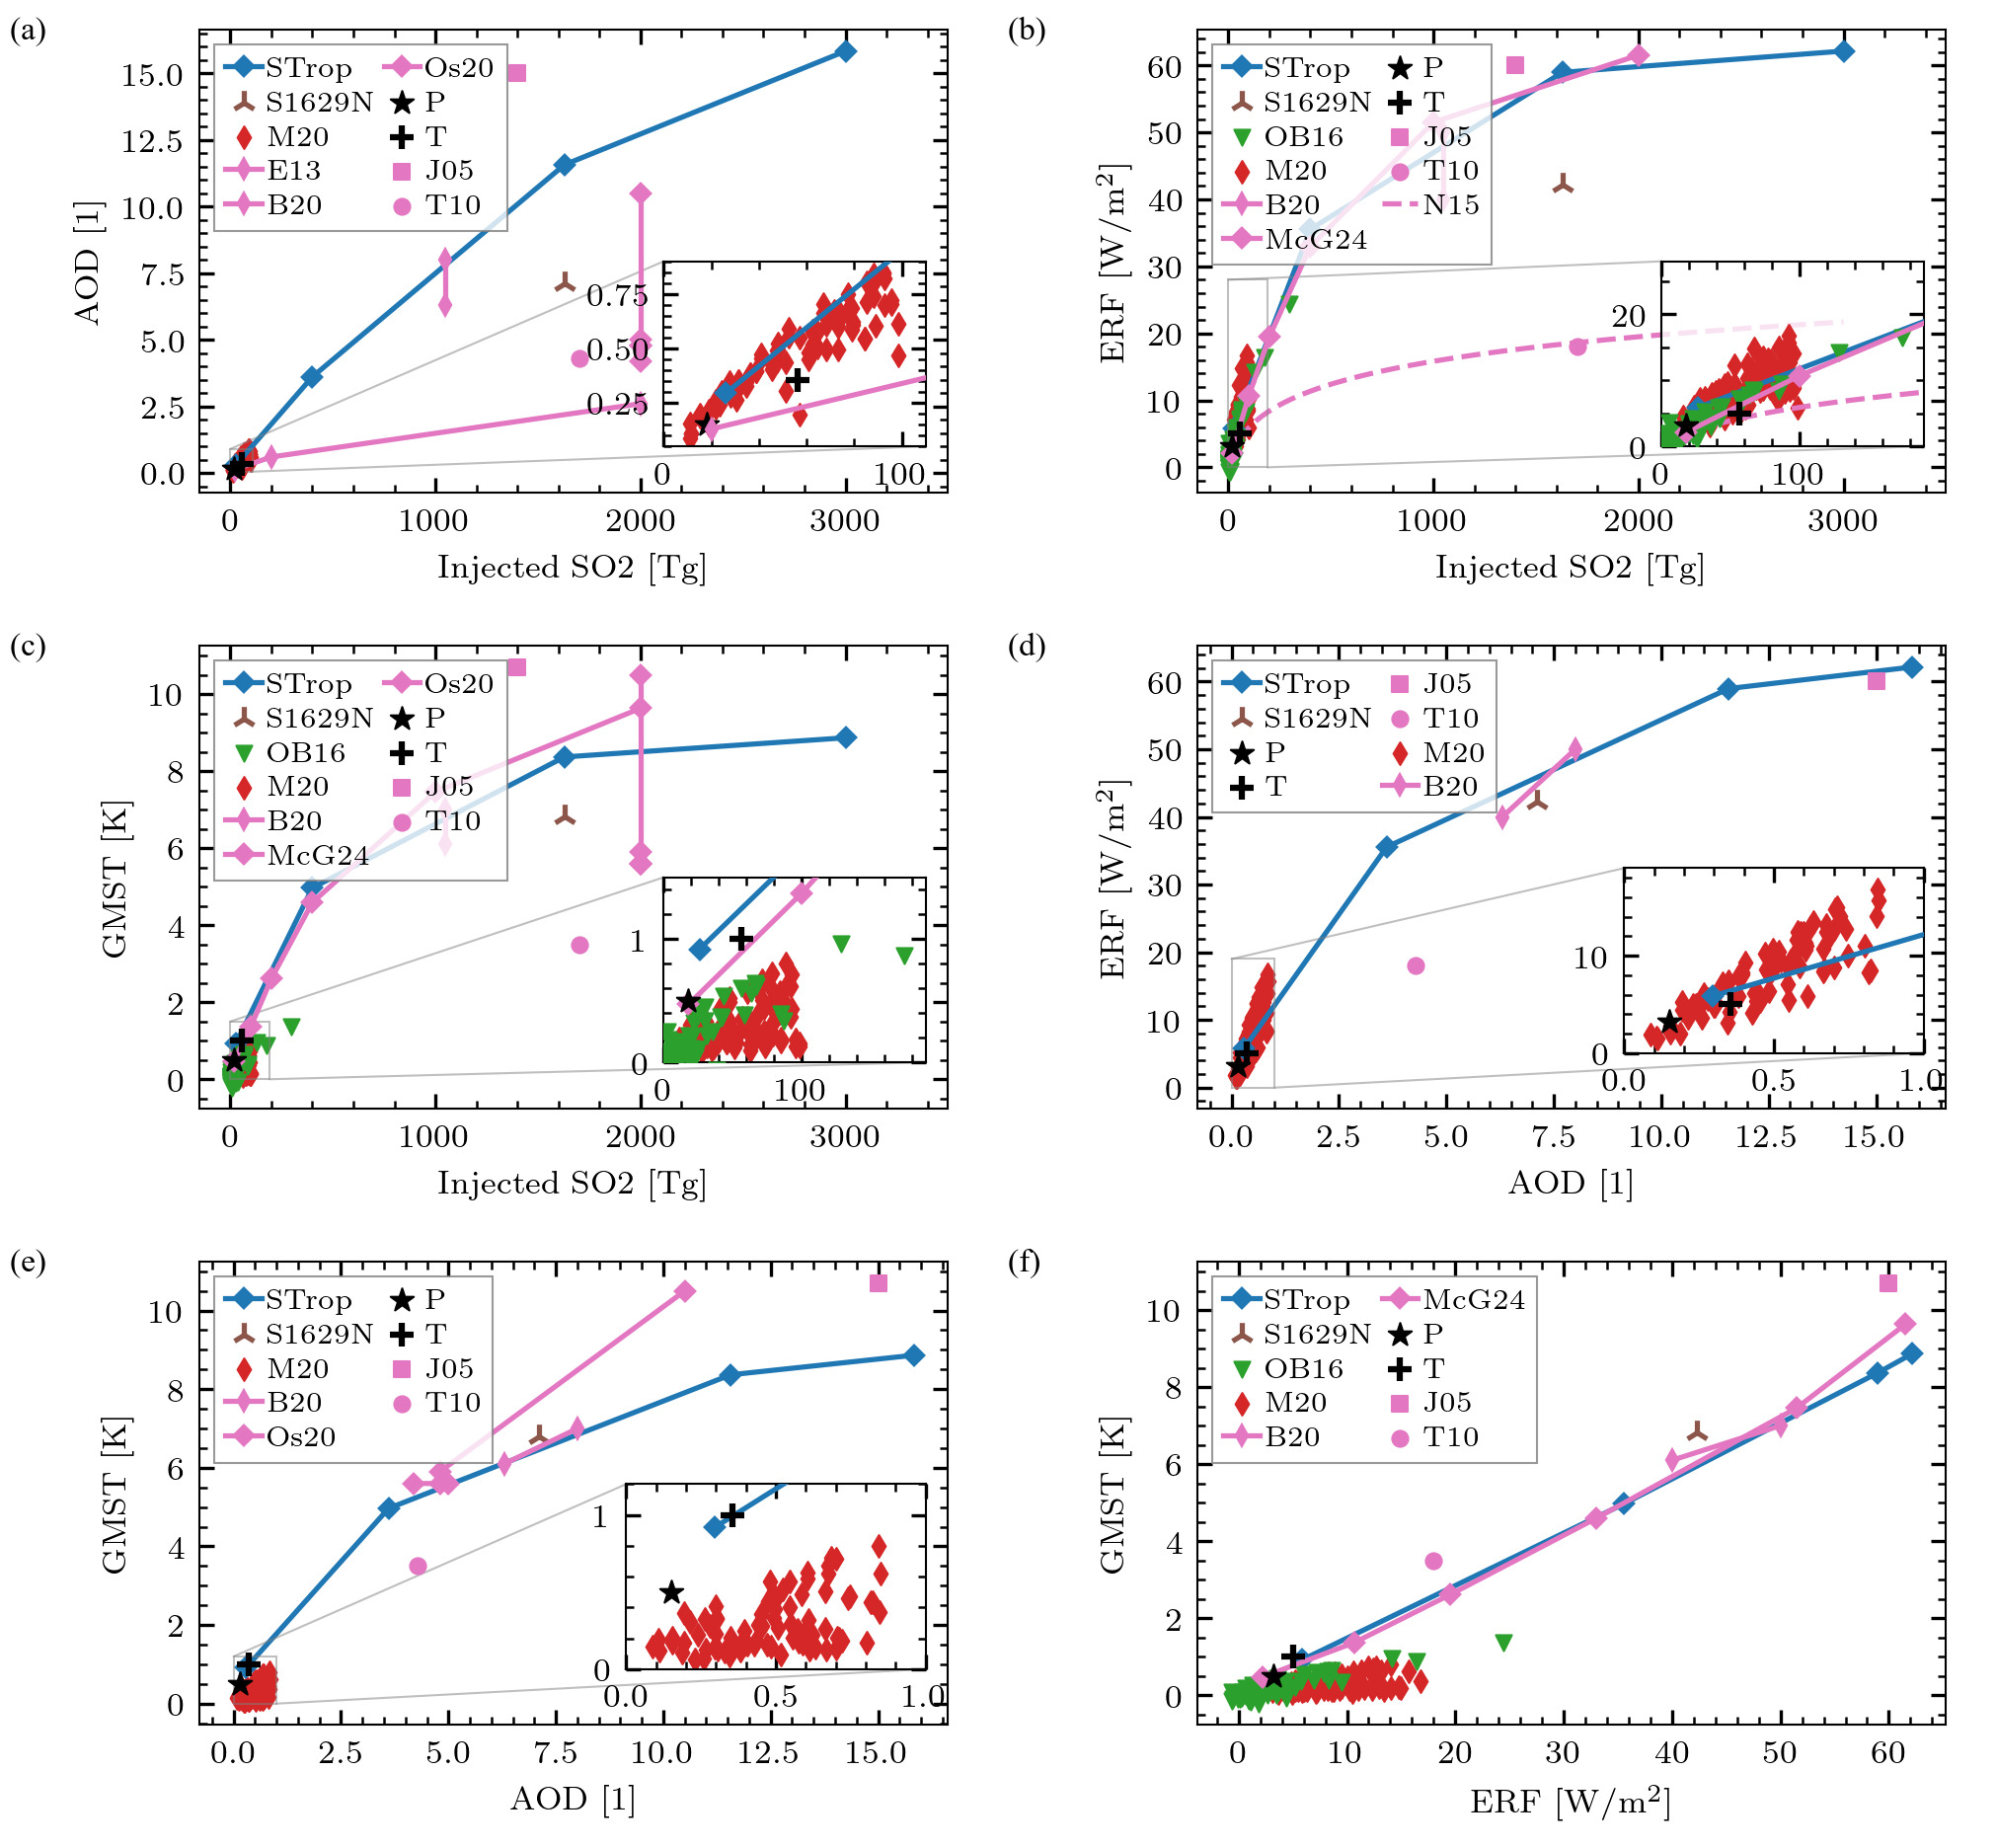
\includegraphics[width=1\linewidth]{figure4}

    \caption{Peak values of (a) AOD, (b) ERF, and (c) GMST as a function of injected
      \ce{SO2}\@. (d) ERF and (e) GMST as a function of AOD. (f) GMST as a function of
      ERF. Blue diamonds labelled STrop represent tropical cases (S26, S400, S1629,
      S3000), the brown three-branched twig signifies the S1629N case, and green
      downward triangles denote OB16 while green upward triangles denote B20. The pink
      square is J05 and the red thin diamonds are M20. McG24 and Os20 are indicated by
      purple upward twigs and orange diamonds, while pink circle and dashed line
      represent T10 and N15. Black star and plus indicate Mt.\ Pinatubo and Mt.\ Tambora
      estimates based on observations, and brown thin diamonds denote E13. The stippled
      grey line represent a two-thirds power-law relationship between AOD and \ce{SO2}
      as suggested by \citeA{crowley2013}. Note that all the data points in the legend
      do not provide all four parameters, and are thus not part of every
      subfigure.}\label{fig:4_parameter_scan}%
  \end{figure*}

  \citeA{niemeier2015} conducted simulations of continuous sulphur injections up to
  \(\SI{200}{\tera\gram(\ce{SO2})\mathrm{yr}^{-1}}\) in the ECHAM5's middle atmosphere
  version \cite{giorgetta2006} with aerosol microphysics from HAM \cite{stier2005}. They
  observed an ERF dependence on \ce{SO2} injection rate following an inverse
  exponential, which converges to \(\SI{-65}{\watt\meter^{-2}}\), depicted in
  Fig.~\ref{fig:4_parameter_scan}b as the stippled pink line labelled N15 and given as;
  \begin{linenomath*}
    \begin{equation}
      \Delta R_{\mathrm{TOA}}(x) = -\SI{65}{\watt\metre^{-2}} \exp\left[-{\left(\frac{\SI{2246}{\tera\gram(S)yr^{-1}}}{x}\right)}^{0.23}\right].
      \label{eq:niemeier_exponential}
    \end{equation}
  \end{linenomath*}
  Here, \(x\) represents injected \ce{S} per year in \(\si{\tera\gram}\), where injected
  mass in \(\si{\tera\gram(\mathrm{SO_{2}})}\) is \(2\times\si{\tera\gram(S)}\). The
  results by N15, on which Eq.~\ref{eq:niemeier_exponential} is based, are all averages
  over at least three years of steady sulphur burdens, substantially longer than the
  time it takes for ERF to reach peak values after an eruption. Combined with their lack
  of a full chemistry model \cite{niemeier2015}, a direct comparison between
  Eq.~\ref{eq:niemeier_exponential} to peak ERF values (occurring about one year
  post-eruption) may not reflect the same chemical and physical processes.

  With these caveats in mind, we observe that even though most simulations exhibit a
  notably faster increase than the exponential relationship, T10's results closely align
  with the function described in Eq.~\ref{eq:niemeier_exponential}. Starting with an
  initial input of \(\SI{850}{\tera\gram(\ce{S})}\) (equivalent to
  \(\SI{1700}{\tera\gram(\ce{SO2})}\), representing the YTT eruption), their estimated
  AOD led to a peak ERF of \(\SI{-18}{\watt\meter^{-2}}\), depicted as a pink filled
  circle in Fig.~\ref{fig:4_parameter_scan}b. The results from T10 came from a
  simulation using the MPI-ESM climate model, driven by AOD data from the HAM aerosol
  model. This alignment likely stems from the utilization of the same aerosol
  microphysical model in both \citeA{timmreck2010} and \citeA{niemeier2015}, as well as
  the application of similar climate models, MPI-ESM and ECHAM5, respectively. The
  relationship between climate model families and their implications are further
  described in Appendix C. Notably, the peak values from M20 align with OB16 and fit
  well within a lower boundary defined by Eq.~\ref{eq:niemeier_exponential}.
  Importantly, none of the eruption simulations shown in
  Fig.~\ref{fig:4_parameter_scan}b exceeded the upper threshold of
  \(\SI{-65}{\watt\meter^{-2}}\) as suggested in Eq.~\ref{eq:niemeier_exponential}.

  Figure~\ref{fig:4_parameter_scan}c illustrates the response of GMST against injected
  \ce{SO2}. The increase in GMST response with injected \ce{SO2} decreases for higher
  injected \ce{SO2}, showing a similar relationship between STrop, S1629N, OB16, B20,
  and McG24. Notably, T10 and J05 exhibit respectively much weaker and much stronger
  GMST responses to injected \ce{SO2} than STrop, while Os20 cover a wide range in GMST
  for the same injceted \ce{SO2} of \(\SI{2000}{\tera\gram(SO_{2})}\). In Os20 they
  removed a single mechanism at the time, with four experiments with GMST between
  \(\SI{5.5}{\kelvin}\) and \(\SI{6}{\kelvin}\), and one at \(\sim \SI{10.5}{\kelvin}\).
  For this outlier, feedback on photochemistry due to aerosols had been switched off
  \cite{osipov2020}. T10 has a maximum GMST anomaly of only \(\SI{-3.5}{\kelvin}\) for
  their \(\SI{1700}{\tera\gram(\ce{SO2})}\) eruption, while J05 records a substantially
  larger maximum GMST anomaly of \(\SI{-10.7}{\kelvin}\). Since the M20 experiment was
  conducted with prescribed sea-surface temperatures \cite{marshall2020}, preventing the
  GMST from being fully perturbed, we do not focus on the M20 data in the GMST plots but
  include them for completeness.

  In Fig.~\ref{fig:4_parameter_scan}d, we revisit the relationship between ERF and AOD,
  focusing on peak values rather than annual and seasonal averages. As previously
  discussed, the ERF to AOD ratio displays weaker slopes than previous studies, with the
  STrop peak values not conforming to a linear trend. The relationship between ERF and
  AOD suggests potential substantial dependencies on the model and its input parameters,
  such as latitude, but most notably to an inherent non-linear ERF dependence on AOD.
  Both the G16 data in Fig.~\ref{fig:2_rf_vs_aod_slopes} and the J05 data originate from
  the same climate model. Similarly to what we find from the STrop data, the ratio is
  much stronger for small eruptions in the industrial era (G16) compared to the
  super-volcano eruption (J05).

  In Fig.~\ref{fig:4_parameter_scan}e, we again find that the response of the STrop data
  increases sublinearly with increasing AOD, this time in GMST anomaly. Additionally,
  both S1629N and B20 align well with STrop, with T10, and J05 and Os20 following a
  similar dependence, albeit somewhat weaker and stronger, respectively. We again note
  the one outlier from Os20 stemming from the simulation where feedback on
  photochemistry due to aerosols was switched off.

  Finally, in Fig.~\ref{fig:4_parameter_scan}f, we compare the GMST and ERF responses.
  STrop show a remarkably linear relationship bewtween GMST and ERF, with most other
  simulations (S1629N, T10, B20, McG24) and observation based estimates (P, T) following
  STrop closely. J05 is also not far off the STrop data, but still represent a small
  deviation from the other estimates. OB16 also show a linear, yet shallower slope as
  compared to STrop, implying stronger GMST perturbations in STrop as compared to OB16.
  However, potential biases exist in the values from the analysis of OB16, as outlined
  in Appendix B, section~\ref{ap:ob16}. This, along with considerable noise, results in
  the analysis of OB16 GMST anomalies being less reliable.

  % The almost linear relationship between AOD and injected \ce{SO2} for the STrop data in
  % Fig.~\ref{fig:4_parameter_scan}a suggests a comparable trend for ERF versus injected
  % \ce{SO2} in Fig.~\ref{fig:4_parameter_scan}b, as seen for ERF versus AOD in
  % Fig.~\ref{fig:4_parameter_scan}d. For the same reason, we expect
  % Fig.~\ref{fig:4_parameter_scan}e to show a similar pattern for STrop as observed in
  % Fig.~\ref{fig:4_parameter_scan}c.

  % This relationship, along with the functional relationships between all other
  % parameters shown in Fig.~\ref{fig:4_parameter_scan}, are illustrated in
  % Fig.~\ref{fig:5_diagram_of_function_relations}. There, \annote[reviewer1]{we show that
  %   from assuming a linear dependency of AOD on injected \protect\ce{SO2}}{why is this
  %   being assumed when it has been shown this isn't very valid?}
  % \annote[reviewer1]{\protect(\(ax+b\)), and of GMST on ERF (\(cx+d\))}{It seems as if x
  %   is referring to different quantities in the different equations. Much more attention
  %   to detail needed if this mathematical framework is to be explained in sufficient
  %   detail.}, we must have that \(f\), \(g\), \(h\), and \(k\) all have the same
  % functional form, where \(f: \ce{SO2} \to \mathrm{ERF}\), \(g: \mathrm{AOD} \to
  % \mathrm{T}\), \(h: \ce{SO2} \to \mathrm{T}\), and \(k: \mathrm{AOD} \to
  % \mathrm{ERF}\). From this, we deduce that \(f(x)=k(ax+b)\) and
  % \(h(x)=f(cx+d)=g(ax+b)\), and finally that \(h(x)=k(acx+ad+b)\), concluding that
  % \(f\), \(g\), \(h\), and \(k\) have the same functional form.

  % \begin{figure}
  %   \centering
  %
  %   \begin{tikzpicture}[>={Stealth[length=1mm,width=2mm]}]
  %     % Place the letters in the corners
  %     \node (A) at (0,0) {AOD};
  %     \node (T) at (4,0) {T};
  %     \node (ERF) at (4,4) {ERF};
  %     \node (S) at (0,4) {\ce{SO2}}; % Draw arrows between the letters
  %     \draw[->] (A) -- node[midway, below] {\(g\)} (T);
  %     \draw[->] (ERF) -- node[midway, right] {\(cx+d\)} (T);
  %     \draw[->] (S) -- node[midway, above] {\(f\)} (ERF);
  %     \draw[->] (S) -- node[midway, left] {\(ax+b\)} (A);
  %     \draw[->] (S) -- node[pos=0.7, above] {\(h\)} (T);
  %     \draw[->] (A) -- node[pos=0.7, above] {\(k\)} (ERF);
  %   \end{tikzpicture}
  %
  %   \caption{Diagram describing the functional relationships of the parameters shown in
  %     Fig.~\ref{fig:4_parameter_scan}.}\label{fig:5_diagram_of_function_relations}%
  % \end{figure}

  \subsection{Climate sensitivity estimate}

  As previously mentioned, the J05 experiment is similar to S1629 concerning ERF values,
  yet differ in both AOD and GMST. At the same time J05 is similar to S3000 in AOD and
  ERF. To investigate this discrepancy, we here conduct a comparison between the J05
  climate feedback parameter \(\alpha\) (where \(s=1/\alpha\) is the climate sensitivity
  parameter) with our climate resistance, denoted as \(\rho\), and the transient climate
  response parameter (TCRP) \(1/\rho\) (where \(\mathrm{TCS}=F_{2\times\ce{CO2}}\times
  \mathrm{TCRP}\) is the transient climate sensitivity and \(F_{2\times\ce{CO2}}\) is
  the forcing due to a doubling of pre-industrial \ce{CO2} concentration). As the
  forcing of volcanic eruptions last for too short time for \(F=\rho T\) to remain
  valid, an alternative approach using a time-integral form introduced by
  \citeA{merlis2014} is applied:

  \begin{linenomath*}
    \begin{equation}
      \int_0^{\tau}F \mathrm{d}t=\rho\int_{0}^{\tau}T \mathrm{d}t
      \label{eq:climate-resistance-orig}
    \end{equation}
  \end{linenomath*}
  \begin{linenomath*}
    \begin{equation}
      \rho=\frac{\int_0^{\tau}F \mathrm{d}t}{\int_{0}^{\tau}T \mathrm{d}t}.
      \label{eq:climate-resistance}
    \end{equation}
  \end{linenomath*}

  If the upper bound of the integral, \(\tau\), is sufficiently large, so that the upper
  ocean heat content is the same at \(t=0\) and \(t=\tau\) (\citeA{merlis2014} used
  \(\tau =\SI{15}{\mathrm{yr}}\)), this approach agrees with \(F=\rho T\) for long-term
  forcing \cite{gregory2016}. Additionally, we note that the climate resistance and the
  climate feedback parameter are associated with the ocean heat uptake efficiency
  (\(\kappa\)) through \(\rho =\alpha +\kappa\) \cite{gregory2016}.

  The climate feedback parameter estimated by \citeA{jones2005} is \(\alpha \simeq
  \SI{4}{\watt\metre^{-2}\kelvin^{-1}}\), exceeding twice the value obtained by
  \citeA{gregory2016} in their simulations of Mt.\ Pinatubo using the same HadCM3
  climate model. We determine the climate resistance using the integral-form computation
  outlined in Eq.~\ref{eq:climate-resistance} and adopting \(\tau
  =\SI{20}{\mathrm{yr}}\). The estimated climate resistance from the three tropical
  simulation cases (with four in each ensemble) converges to \(\rho
  =\SI{2.5(4)}{\watt\metre^{-2}\kelvin^{-1}}\), and TCRP values of
  \(1/\rho=\SI{0.41(5)}{\kelvin\watt^{-1}\metre^{2}}\), as reported in
  table~\ref{tab:trcp}, and is therefore assumed to be a good estimate of \(\alpha\).

  Importantly, our estimate agrees well with G16, while the J05 estimate of \(\alpha
  \simeq \SI{4}{\watt\metre^{-2}\kelvin^{-1}}\) is still notably higher. Since the GMST
  perturbation obtained by J05 was larger than in any of our STrop cases, it indicates
  that the forcing used by J05 must be stronger. The peak value of the J05 ERF is
  similar to the S1629 case, and as such, the overall stronger forcing must originate
  from the development of the forcing time series rather than the peak value. This is in
  line with previous results showing that from larger eruptions, the aerosol effective
  radius peak increase, as well as the aerosol effective radius experiencing a shorter
  \(e\)-folding time \cite{clyne2021}. This result in a sharper peak in AOD and ERF,
  with the peak values increasing sublinearly with increasing \ce{SO2}
  \cite{english2013,timmreck2009,zanchettin2016,clyne2021}. In addition, \ce{OH}
  scarcity is assumed to limit the \ce{SO2} oxidation, delaying the AOD peak for
  sufficiently large eruptions \cite{timmreck2010}. Further, \citeA{mcgraw2024} find
  that from supereruptions, it is possible to achieve even a warming of the GMST by
  fixing the aerosol effective radius to \(R_{\mathrm{EFF}}>\SI{2.5}{\micro\meter}\). As
  our model results align well with the results of \citeA{mcgraw2024} using a small
  aerosol effective radius of \(R_{\mathrm{EFF}}=\SI{0.6}{\micro\meter}\), we expect the
  peak GMST from CESM2(WACCM6) to be close to a lower (cooling) bound, and as such that
  the even colder GMST perturbation of \citeA{jones2005} is too extreme.

  \begin{table}
    \centering

    \caption{Estimated climate resistance and TCRP\(^{a}\)}\label{tab:trcp}%
    \begin{tabular}{ccc}
      \toprule
      Simulation type & \(\rho [\si{\watt\metre^{-2}\kelvin^{-1}}]\) & \(1/\rho\) \\
      \midrule
      S1629 & \(\num{2.21\pm0.05}\) & \(\num{0.45\pm0.01}\) \\
      S400 & \(\num{2.51\pm0.06}\) & \(\num{0.40\pm0.01}\) \\
      S26 & \(\num{2.9\pm0.6}\) & \(\num{0.36\pm0.07}\) \\
      Total & \(\num{2.5\pm0.4}\) & \(\num{0.41\pm0.05}\) \\
      \toprule
      \multicolumn{3}{l}{\parbox{0.5\linewidth}{\(^{a}\)Estimates are based on ensembles with four members and \(\tau
          =\SI{20}{\mathrm{yr}}\) using Eq.~\ref{eq:climate-resistance}.}} \\
    \end{tabular}
  \end{table}

  \section{Discussion}

  \label{sec:discussion}

  % NOTE: Suggested layout for the
  % Discussion:
  % - Explain the results and emphasize significant findings clearly
  % - Discuss the impact and importance of results compared with recent relevant research
  % Conclusion
  % - The justification for these objectives: Why is the work important?
  % - Summarize the key points made in the other sections
  % - Conclude overall discussion of article
  % - Link this section to the introduction

  % ERF / AOD linearity does not hold for large eruptions
  Figures~\ref{fig:2_rf_vs_aod_slopes},~\ref{fig:3_rf_to_aod_ratios}, and
  \ref{fig:4_parameter_scan}d demonstrate that as the AOD exceeds approximately \(1.0\),
  the linear ERF dependence of approximately
  \(\SI{-20}{\watt\metre^{-2}\mathrm{AOD}^{-1}}\) no longer holds. The sublinear
  increase in ERF with injected \ce{SO2} in Fig.~\ref{fig:4_parameter_scan}b for large
  eruptions is consistent with previous results from simulations using similar climate
  models of smaller historic eruptions (G16) and of supereruptions (J05). Such a change
  in ratio has been attributed to larger eruptions, injecting more \ce{SO2}, leading to
  larger aerosols, and hence less effective radiation scattering, thereby reducing the
  ERF for the same injected \ce{SO2} \cite{english2013, timmreck2010, timmreck2018}.
  Similarly, previous studies have suggested a two-thirds power law relationship between
  peek AOD and injected \ce{SO2} for eruptions larger in magnitude than than the Mt.\
  Tambora eruption \cite{crowley2013,metzner2014,timmreck2024}. Furthermore, CESM(WACCM)
  has been shown to simulate smaller aerosols than most other climate models
  \cite{clyne2021}, resulting in an increased AOD peak value and longer \(e\)-folding
  time \cite{zanchettin2016,clyne2021}. Thus, the sublinear relationship for AOD and ERF
  to injected \ce{SO2} from CESM2(WACCM6) is likely an upper bound.

  % Latitude is more important for the development of the ERF / AOD ratio
  The non-linear relationship between peak ERF and AOD values is a strong signature in
  both Figs.~\ref{fig:2_rf_vs_aod_slopes} and~\ref{fig:3_rf_to_aod_ratios}. Across
  eruptions of the same strength, the ratio stays relatively constant, leading to a
  close to \(\SI{-10}{\watt\metre^{-2}\mathrm{AOD}^{-1}}\) slope for S400 and a
  \(\SI{-5}{\watt\metre^{-2}\mathrm{AOD}^{-1}}\) slope for S1629 and S3000. Still, a
  non-linear development in the ERF to AOD ratio is found across all tropical eruptions.
  Similar to the results of \citeA{marshall2020}, we find in S400, S1629, and S3000 that
  the post-peak period (second and third post-eruption years) has a stronger aerosol
  forcing efficiency compared to the pre-peak period (first post-eruption year). The
  post-peak period of S26 is elevated as compared to the pre-peak period, resulting in a
  decreasing aerosol forcing efficiency from the first to the second and third
  post-eruption years, in contrast to the other tropical eruptions.

  Focusing on the pre-peak period, we find tropical eruptions to differ from eruptions
  at high latitudes. During the pre-peak period, all tropical eruptions show a
  decreasing aerosol forcing efficiency, while no significant change in the ERF to AOD
  ratio is found from the S1629N case. The full M20 dataset indicates an increasing
  aerosol forcing efficiency also during the pre-peak period, contrasting the decreasing
  efficiency found from their tropical eruptions and supporting the latitudinal
  dependence we find with S1629N. While we find a linear relationship to be a useful
  approximation of ERF dependence on AOD for eruptions similar to or smaller than Mt.\
  Pinatubo, additional factors must be considered for larger eruptions. These factors,
  such as \ce{OH} scarcity contributing to delayed \ce{SO2} oxidation, and aerosol
  growth influencing reflectance and their gravitational pull, substantially impact both
  AOD and ERF evolution, as highlighted by \citeA{timmreck2010}. The large difference in
  ratio found when comparing eruption magnitudes suggests that injected \ce{SO2} is
  crucial when estimating the time-average of the ERF to AOD ratio. However, latitude
  and, in particular, aerosol dispersion are more influential in determining the
  post-eruption evolution of the ratio, particularly during the pre-peak period.

  We find that the suggested upper threshold from Eq.~\ref{eq:niemeier_exponential} is
  not violated by any eruption simulation, and most notably that the GMST peak value
  follow the ERF trend in reaching a limiting value. The STrop cases follow a close to
  linear GMST dependency on ERF, with S1629N, T10, B20, and McG24 all aligning close to
  the same slope. The linear relationship between GMST and ERF is the strongest
  dependence found between the parameters in Fig.~\ref{fig:4_parameter_scan}, and a
  strong signature across both eruption magnitudes and latitudes, but also across highly
  different climate models. Thus, from a maximum ERF of \(\SI{-65}{\watt\metre^{-2}}\),
  we expect GMST anomalies to reach at most \(\sim\SI{-10}{\kelvin}\), in support of
  \citeA{english2013} who suggested that large eruptions can be self-limiting. While J05
  achieve an even stronger cooling, the long \(e\)-folding time of their AOD time series
  is believed to contribute a too strong forcing and climate feedback parameter,
  resulting in an estimated GMST that is too extreme.

  % Models vary in their SO2 to H2SO4 chemistry/physics, but are comparatively
  % consistent in representing AOD, ERF and GMST.
  The biggest spread in the data shown in Fig.~\ref{fig:4_parameter_scan} is found when
  relating injected \ce{SO2} to any of the three output parameters. Computing the
  Pearson correlation coefficient for the data in Fig.~\ref{fig:4_parameter_scan}
  (except OB16 and M20, as they provide many more data points compared to all other and
  would skew the correlation) equates to \(0.670\), \(0.799\), and \(0.758\) for
  injected \ce{SO2} against AOD, RF, and GMST, respectively. In comparison, coefficients
  for AOD against ERF, AOD against GMST, and ERF against GMST equals \(0.946\),
  \(0.918\), and \(0.986\). The AOD to injected \ce{SO2} relationship is consistent
  within similar models, even when comparing simulations of volcanic eruptions
  \cite{timmreck2010} and continuous injection of \ce{SO2} \cite{niemeier2015}, but has
  a wide spread at high values of injected \ce{SO2} across model families
  (Figs.~\ref{fig:4_parameter_scan}a,b,c). Comparatively, the ERF
  (Fig.~\ref{fig:4_parameter_scan}d) and GMST (Fig.~\ref{fig:4_parameter_scan}e) as a
  function of AOD, as well as GMST as a function of ERF
  (Fig.~\ref{fig:4_parameter_scan}f), demonstrate a smaller spread across models.
  \citeA{marshall2019, marshall2020, marshall2021} use a code with seven log-normal
  modes to simulate aerosol mass and number concentrations, along with an
  atmosphere-only configuration of the UM-UKCA with prescribed sea-surface temperatures
  and sea-ice extent \cite{marshall2019}. This approach is in contrast with CESM2,
  operating as an Earth System Model, but with a simpler aerosol chemistry model in the
  MAM3. The family of models to which M20 is based is different from that of STrop,
  OB16, E13, and B20, with T10 and N15, and Os20 and McG24 from yet two more model
  families, as described in Appendix C. Based on Fig.~\ref{fig:4_parameter_scan}, we
  find the model family to be pivotal in determining the estimated AOD and ERF
  magnitudes from injected \ce{SO2}, whereas the various models generally demonstrate
  more consistency in representing ERF from AOD.

  \section{Summary and conclusions}

  \label{sec:conclusions}

  We consider five ensembles of Mt.\ Pinatubo-sized to supereruption sized events and
  compare them to previously reported results. We find the commonly adopted ERF
  dependence on AOD of \(\sim\SI{-20}{\watt\metre^{-2}\mathrm{AOD}^{-1}}\) to be
  representative for Mt.\
  Pinatubo-sized eruptions. Larger eruptions, with one to two orders of magnitude larger
  injections of \ce{SO2}, are found to have an ERF dependence on AOD closer to
  \(\sim\SI{-10}{\watt\metre^{-2}\mathrm{AOD}^{-1}}\) and
  \(\sim\SI{-5}{\watt\metre^{-2}\mathrm{AOD}^{-1}}\). A shallower slope for larger
  eruptions is also consistent with peak values from previous studies of supereruptions.

  The time-after-eruption dependence of the ratio between ERF and AOD is found to weaken
  with time, resulting in a decreasing aerosol forcing efficiency in the pre-peak
  period. The effect is found across all eruption sizes, but only the tropical cases
  show a clear trend. The high-latitude case displays an almost constant efficiency with
  time. These results agree with a reanalysis of the tropical data in
  \citeA{marshall2020dataset}. Thus, these findings provide strong supporting evidence
  that latitude is generally significant in determining the aerosol forcing efficiency,
  particularly as a function of time-after-eruption. These findings emphasise the
  complexity of volcanic impacts on climate, demonstrating significant differences in
  climatic response depending on eruption magnitude and latitude.

  A clear trend across all simulations performed here and across several previous
  studies is a linear relationship between peek GMST and ERF. Further, the peak values
  seem to stagnate with no ERF peaks breaking the suggested lower bound of
  \(\text{ERF}=\SI{-65}{\watt\metre^{-2}}\) by \citeA{niemeier2015}. Thus, we expect
  supereruptions to be self-limiting with the most extreme GMST perturbations reaching
  at most \(~\sim \SI{-10}{\kelvin}\).

  We find that the AOD peak arrives later for larger eruptions than for smaller ones,
  and also that larger eruptions produce a sharper peak in the AOD time series. The ERF
  time series are similar across all eruption sizes, and while the smallest eruption
  experiences a faster GMST decay, the larger eruptions produce time series
  indistinguishable in development for both ERF and GMST. Thus, a simple scaling of the
  AOD or GMST time series from a smaller eruption is insufficient in representing that
  of larger volcanic eruptions.

  Considering injected \ce{SO2} and the peak values of AOD and ERF, a large spread is
  found across model families in Fig.~\ref{fig:4_parameter_scan}. Improving the
  consistency between model families in how the chemistry and physics of aerosols are
  represented is an important step in enhancing the accuracy of simulated volcanic
  eruptions' influence on climate by models. More simulations of larger volcanic
  eruptions with injected \ce{SO2} greater than \(\SI{200}{\tera\gram(\mathrm{SO2})}\)
  would provide useful information for a more precise determination of the ERF to AOD
  ratio in the non-linear regime. This would also serve as a useful test to check if a
  comparison between \ce{SO2} injection events and continuous \ce{SO2} injection is
  reasonable. Introducing a spread in latitude similar to the
  \citeA{marshall2020dataset} dataset would allow for better comparison between
  eruptions across all latitudes and the suggested lower limit following
  Eq.~\ref{eq:niemeier_exponential}, describing a situation of aerosol saturation.

  \appendix

  \section{Simulation setup}

  Input files used in the simulations were created by modifying the file available at \url{http://svn.code.sf.net/p/codescripts/code/trunk/ncl/emission/createVolcEruptV3.ncl},
  using a Python package available on GitHub at
  \url{https://github.com/engeir/volcano-cooking} or through the Python Package Index
  (PyPI). The package is available both as a library and a Command Line Interface (CLI),
  and is used to create volcanic eruptions with a specified amount of \ce{SO2} that is
  injected over six hours at a given latitude, longitude, and altitude. All volcanic
  \ce{SO2} files are created from a shell script by setting the eruption details in a
  JSON file that is read by the \texttt{volcano-cooking} CLI at a fixed version,
  ensuring a reproducible experiment setup.

  During analysis, one outlier was found in the ensemble representing S26, specifically
  in the GMST time series. This ensemble member was the February 15, 1850, eruption,
  which was changed in favour of a February 15, 1851, eruption in the S26, S400, and
  S1629 ensembles. For completeness, the February 15, 1850, eruption is still included
  in the online archive.

  \section{External data}

  \subsection{Otto-Bliesner data analysis}

  \label{ap:ob16}

  Data from \citeA{ottobliesner2016} are the original input data of injected \ce{SO2} as
  used in their model simulations, along with ERF and GMST output data. The injected
  \ce{SO2} can be found at
  \url{https://www.cesm.ucar.edu/working-groups/paleo/simulations/ccsm4-lm}. Only the
  peak values of the \ce{SO2} dataset were used in the analysis. Output variables are
  available at \url{www2.cesm.ucar.edu/models/experiments/LME}.

  Since the OB16 dataset contains a five-member ensemble, the final ERF and GMST time
  series used were ensemble means. A single control simulation time series is used to
  remove seasonal dependence from the GMST, where the control simulation is averaged
  into a climatology mean. Further, a drift in the GMST is removed by subtracting a
  linear regression fit. ERF has seasonality removed in the Fourier domain.

  The time of an eruption is found based on a best attempt at aligning the \ce{SO2} time
  series with both the ERF time series and the GMST time series. The ERF and GMST peak
  values are taken as the value of the time series at the time of an eruption according
  to the \ce{SO2} time series. Missing the true peak means the found peaks will be
  biased towards lower values. However, instances where eruptions occur close in time
  will contribute a bias to higher values. These biases contribute to a greater
  uncertainty related to OB16 in Figs.~\ref{fig:4_parameter_scan}b,c,f.

  \subsection{Marshall data analysis}

  \label{ap:m20}

  Data used to compute the M20 values were from \citeA{marshall2020dataset}, available
  at \url{https://doi.org/10.5285/232164e8b1444978a41f2acf8bbbfe91}. As each file
  includes a single eruption, peak values of AOD, ERF, and GMST were found by applying a
  Savitzky-Golay filter of third order and one-year window length, and choosing the
  maximum value \cite{savitzky1964}.

  \subsection{Gregory data analysis}

  \label{ap:g16}

  Data used to compute G16 values were kindly provided by Jonathan Gregory (personal
  communication). This include a 160-year long simulation with the HadCM3 using the
  sstPiHistVol simulation set-up, specifying a fixed sea-surface temperature simulation
  of historic volcanoes in pre-industrial conditions. The full 160-year-long time series
  were further analysed by computing annual means.

  \section{Model families}

  The model used here was the CESM2 with the WACCM6 atmosphere in the MA configuration.
  The MA configuration uses the MAM3 \cite{gettleman2019}, a simplified and
  computationally efficient default setting within the CAM5 \cite{liu2016}, as described
  in \citeA{liu2012}. The MAM3 was developed from MAM7, consisting of the seven modes
  Aitken, accumulation, primary carbon, fine dust, fine sea salt, coarse dust, and
  coarse sea salt. Instantaneous internal mixing of primary carbonaceous aerosols with
  secondary aerosols and instantaneous ageing of primary carbonaceous particles are
  assumed by emitting primary carbon in the accumulation mode \cite{liu2016}. As dust
  absorbs water efficiently and is expected to be removed by wet deposition similarly to
  sea salt, fine dust is merged with fine sea salt into the accumulation mode and coarse
  dust is merged with coarse sea salt into a coarse mode. The coarse mode will quickly
  revert to its background state below the tropopause \cite{liu2012}. Consequently, MAM3
  features the three modes Aitken, accumulation, and coarse \cite{liu2016}.

  The CESM2 is an ancestor of CESM1 used by OB16. They belong to a different model
  family than both the HadCM3 (J05 and G16) and the UM-UKCA (M20), which is an extended
  version of HadGEM3 \cite{dhomse2014}, and an ancestor of HadCM3. A third model family
  is represented through ECHAM5 (N15) and MPI-ESM (T10), where the latter is related to
  the former via the ECHAM6. Finally, a fourth family is represented through the GISS
  ModelE2.1 used by both Os20 and McG24. A summary of the model code genealogy is in
  table~\ref{tab:model-family}, based on the model code genealogy map created by
  \citeA{kuma2023}.

  \begin{table*}
    \centering
    \caption{Model code family relations\(^{a}\)}\label{tab:model-family}

    \begin{tabular}{ccc}
      \toprule
      Family relation & Model name & Data name \\
      \midrule
      \multirow{2}{*}{CESM1 \(\rightarrow\) CESM1-CAM5 \(\rightarrow\) CESM2}
      & CESM1 & E13\(^\ast\), OB16 \\
      & CESM2 & B20, \emph{This contribution} \\
      % ---
      & HadCM3 & J05, G16 \\
      \multirow{-2}{*}{\shortstack{HadCM3 \(\rightarrow\) HadGEM1
          \(\rightarrow\) \\
          HadGEM2 \(\rightarrow\) HadGEM3 \(\rightarrow\) UM-UKCA}} & UM-UKCA &
      M20 \\
      % ---
      \multirow{2}{*}{ECHAM5 \(\rightarrow\) ECHAM6 \(\rightarrow\) MPI-ESM}
      & ECHAM5 & N15 \\
      & MPI-ESM & T10 \\
      GISS-E2.1 & GISS ModelE2.1 & Os20, McG24 \\
      \toprule
      \multicolumn{3}{l}{\parbox{\linewidth}{\(^{a}\)Overview of various model codes
          grouped into families according to the model code genealogy map by
          \citeA{kuma2023}, with each table entry also indicating the specific model
          code used in the referenced papers of this study. \(^\ast\)The E13 simulation used
          WACCM3, only simulating the atmosphere, but falls into the same family of models
          as OB16, B20 and this contribution.}} \\
    \end{tabular}
  \end{table*}

  %% NOTE that acronyms in the final published version will be spelled out when used in figure captions.
  \begin{acronyms}
    \acro{AODVISstdn} ``stratospheric aerosol optical depth 550 nm day night''
    \acro{AOD} stratospheric aerosol optical depth \acro{CAM5} Community Atmosphere
    Model Version 5 \acro{CESM1} Community Earth System Model Version 1 \acro{CESM2}
    Community Earth System Model Version 2 \acro{ECS} equilibrium climate sensitivity
    \acro{ERF} effective radiative forcing \acro{FLNT} ``net longwave flux at the top of
    the model'' \acro{FSNT} ``net solar flux at the top of the model'' \acro{GMST}
    global mean surface temperature \acro{IRF} instantaneous radiative forcing
    \acro{MAM3} three mode version of the Modal Aerosol Module \acro{MA} middle
    atmosphere \acro{POP2} Parallel Ocean Program Version 2 \acro{ERF} effective
    radiative forcing \acro{TCRP} transient climate response parameter \acro{TOA}
    top-of-the-atmosphere \acro{TREFHT} ``reference height temperature'' \acro{WACCM6}
    Whole Atmosphere Community Climate Model Version 6 \acro{YTT} Young Toba Tuff
  \end{acronyms}

  \section*{Open Research Section}

  % This section MUST contain a statement that describes where the data supporting the
  % conclusions can be obtained. Data cannot be listed as ''Available from authors'' or
  % stored solely in supporting information. Citations to archived data should be included
  % in your reference list. Wiley will publish it as a separate section on the paper’s page.
  % Examples and complete information are here: https://www.agu.org/Publish with
  % AGU/Publish/Author Resources/Data for Authors

  The direct output data of CESM2 are too large to be easily archived and transferred.
  Instead, data generated directly from output fields of CESM2 are made available in a
  NIRD Research Data Archive \cite{enger2024:nirddataarchive}, and were generated using
  scripts hosted on GitHub and published to Zenodo \cite{enger2024:data-aggregate}.
  Analysis scripts are hosted on GitHub and published to Zenodo
  \cite{enger2024:code4paper1}, with the source code used to generate CESM2 input files
  also hosted on GitHub and published to Zenodo \cite{enger2024:volcano-setup}.

  \acknowledgments

  The simulations were performed on resources provided by Sigma2 --- the National
  Infrastructure for High Performance Computing and Data Storage in Norway.

  This work was supported by the Tromsø Research Foundation under Grant Number
  19\_SG\_AT.

  Thanks to both Maria Rugenstein and Martin Rypdal for valuable discussions. We would
  also like to thank the authors of \citeA{gregory2016}, \citeA{ottobliesner2016}, and
  \citeA{marshall2020dataset} for making their data available.

  \bibliography{agujournaltemplate}

\end{document}
